Arbitration is an application where we select the best among multiple simultaneous ASR results. We explain our arbitration framework for personal assistant experience on smart devices in Fig.~\ref{Fig:Arbitration}. We decode an utterance simultaneously for both client and service engines. Client engine is designed to work with traditional client scenarios like \emph{call, digit dialing, text, open applications etc.}, service engine works better for rest of the speech scenarios including \emph{voice-search, weather etc.}. By design client and service cater seamlessly to all speech scenarios and contain language-model (LM) and acoustic-model (AM) optimized for respective tasks. Though we have distinct engines for client and service speech scenarios, they work together in a unified way that is indistinct for the user as we obviously don't expect user to provide us inputs on his scenario being one of client or service. Arbitration is the key speech application that provides a unified experience by selecting the best among the client and service results.  In Fig.~\ref{Fig:Arbitration} both client and service listen to speech from potentially all scenarios and produce respective recognition results under the constraint of their respective engine, AM and LM. These results are communicated to arbitration where it selects the best between the two results. Arbitration sends the results back to client where a decision unit at client will typically provide the arbitrated result to the user on their smart devices.

There can be a few scenarios where the decision unit can simply choose the client recognition \emph{e.g.}, (a) if client confidence-scores are higher than a present threshold; client can simply choose client ASR result if it's very confident, this avoids latency incurred in hearing back from service and arbitration, (b) in absence of connection to service, then user can still use client side speech applications. %Microsoft or other $3^{rd}$-party applications.

% This framework also allows us to cater to scenarios where a user says: ``text Alex, I will be late". There client engine has access to contacts and can recognize the person name ``Alex" and produce a result like ``text Alex ...", then ``..." will be filled in by recognition from service. Client AM contains garbage paths that greatly help absorb utterances are intended for service only and thus are out-of-grammar (OOG) for client.

%\subsection{Arbitration Classifier and Baseline Features}\label{Sec:ArbitrationCC}
%Brief description of current arbitration framework, and current useful features

\begin{figure}[h]
\centering
{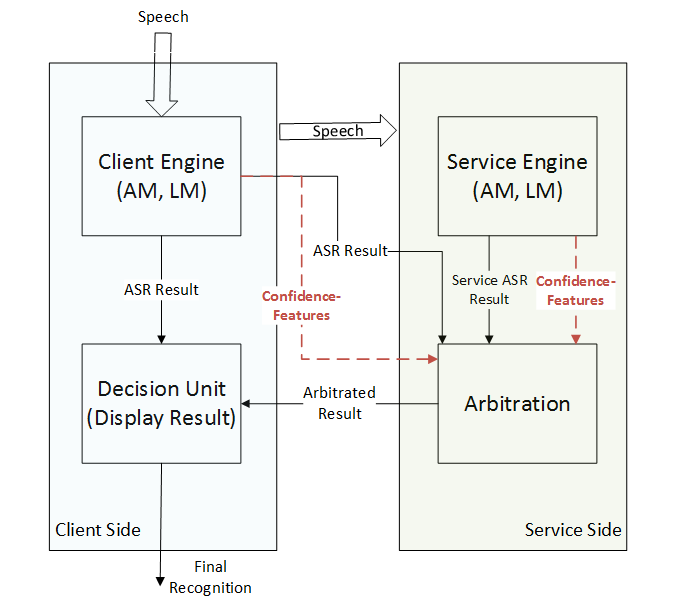
\includegraphics[width=0.48\textwidth]{Arbitration}}
\caption{\it Arbitration for client and service ASR results. We additionally feed confidence-features from both client and server to arbitration.}
\label{Fig:Arbitration}
\end{figure}

\subsection{Incorporating Confidence-Features in Arbitration}
% We described our arbitration framework and the baseline features in \ref{Sec:ArbitrationCC}, there we mentioned a number of features that we found very relevant for arbitration. 

In this section, we build a thesis on consuming the rich set of confidence-features in arbitration. 
Our baseline arbitration is trained from a number of carefully designed features, still the confidence-features provide detailed and complementary information in noise, silence, acoustic and language-model scores, and is expected to be useful for arbitration. Confidence-scores from both client and service are currently used by arbitration, these scores provide a good gist of confidence-features but we can benefit a great deal with directly consuming confidence-features by (a) using much more gradual information in terms of 20-dim confidence-features versus a single confidence-score in arbitration, (b) confidence-scores are designed to optimize the performance of confidence-classifier which is clearly different from arbitration, so retraining with confidence-features helps, (c) arbitration and confidence-classifier may be trained over different datasets, so the information encapsulated by confidence-score may not generalize to dataset relevant for arbitration, (d) confidence-scores are language-specific as they may have been individually trained across a set of \emph{AM, LM, languages, dataset}, in contrast, we have noted that the various inherent normalizations in confidence-features make them robust across locals, so consuming confidence-features can allow us to build an arbitration classifier from one local that can provide good performance for other unseen locals; this can be specially useful when we bootstrap arbitration for a local under limited data scenarios, (e) using confidence-score in arbitration creates a dependency for arbitration on confidences, any update to confidence-classifiers potentially requires retraining arbitration; we can completely alleviate this issue if we consume confidence-features instead of confidence-score in arbitration, this lets us independently update confidence-classifier without impacting arbitration.

We demonstrate our approach that uses the rich confidence-features for arbitration in Fig.~\ref{Fig:Arbitration}. We build the infrastructure required to extract confidence-features from both client and service engine, and communicate them to arbitration, see Fig.~\ref{Fig:Arbitration}. As expected we require little additional work in communicating service confidence-features to arbitration. For client, we additionally send about 30 Bytes-per-second of data, this is less than 0.2\% relative increase to our payload from client to service. Depending on application and need, arbitration can be retrained and deployed with confidence-features from (a) just client, (b) just service, (c) both client and service. 

% 3 second, 20 float features = 20 * 4 = 80 bytes = 30bytes/sec
% speech data = 8000 bytes

\subsection{Arbitration Experiments and Results}\label{Sec:ArbitrationResults}
We present and analyze results with using confidence-features in arbitration.
Our arbitration module was trained from over 35k speech utterances. Testing was done on over 25k utterances. We decoded these utterances against both client and service engines with their respective  AM and LM, and obtained corresponding recognition results. We had ground-truth transcriptions for these utterances and created their classification targets in terms of client or service based on what provided a lower word-error rate. Our baseline arbitration features are 20-dim, that include duration, confidence-score and few semantic features etc. We additionally obtained 20-dim confidence-features from each of client and service. We followed the existing framework for training arbitration that uses a boosted-decision-tree for classification.

% Note that ideally clients will have distinct personalized grammars with their own contact names, application names etc. 

% where we additionally included 20 confidence-features. 

%For our purposes we simulated client grammar with each over 250 names in contacts and used these grammars in decoding. 

We demonstrate the value in client confidence-features in Fig.~\ref{Fig:PhrasePreds-Hist}. There we plot probability-distribution-function for a few features for arbitration task. There ``correct" refers to cases where client wins, and ``InCorrect" refers to service wins, ``Confidence-Score" indicates usual client confidence-score. We visually see that some of the features better separate the 2 classes than confidence-score.

\begin{figure}[h]
\centering
{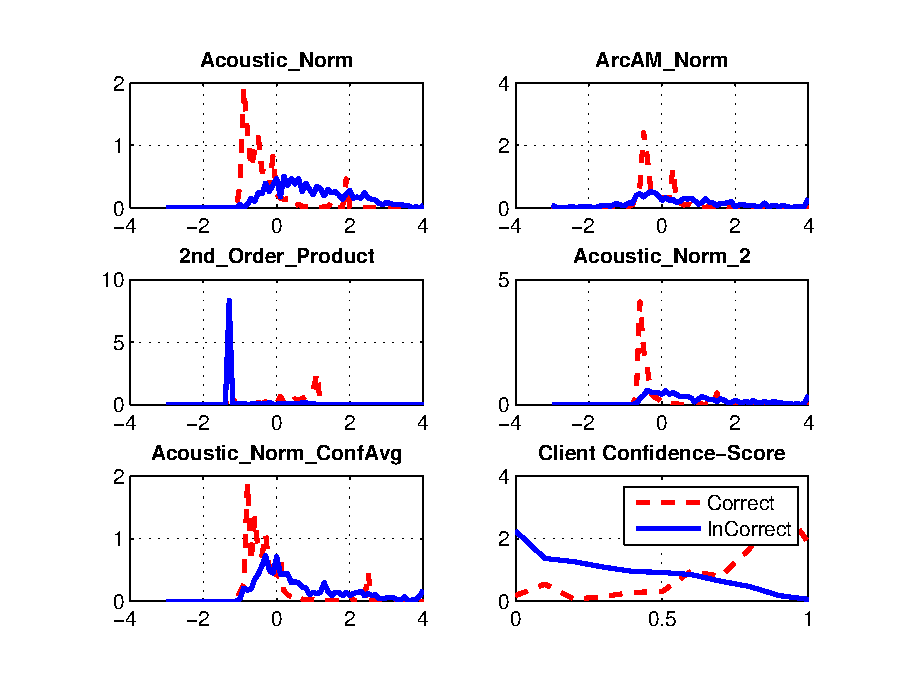
\includegraphics[width=0.45\textwidth]{PhrasePreds-Hist.eps}}
\caption{\it Probability-distribution of representative confidence-features for arbitration.}
\label{Fig:PhrasePreds-Hist}
\end{figure}

Next we provide receiver-operating-curve (ROC) for baseline and with including client confidence-features in Fig.~\ref{Fig:Baseline-ClientPred-ROC}, where we note a strongly better ROC curve throughout the range of curve. In this arbitration task, ``False Positive" (FP) indicates incorrect wins from client and ``True Positive" (TP) indicates correct wins from service. Specifically at FP of 0.1, we can improve TP from 0.81 to 0.86, for a 26\% relative reduction in (1-TP). We note correct area-under-the-curve (AUC) metrics in Table~\ref{tab:AUC_ROC}, where including client confidence-features improved AUC from 0.927 for baseline to 0.946, additionally including server confidence-features improved AUC to 0.95 for a 31.5\% relative reduction in (1-AUC) metric. Our arbitration-classifier ranks all of it's features in the order of importance. As expected confidence-features appear prominently among the top features, with 7 of the top-10 overall features being confidence-features. This further demonstrates that the proposed features outperform and add value to the baseline features.

\begin{figure}[h]
\centering
{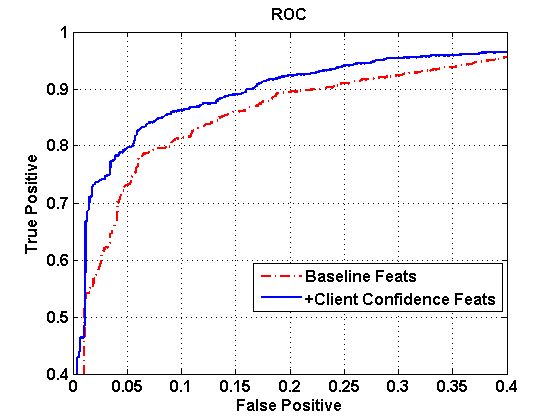
\includegraphics[width=0.4\textwidth]{Baseline-ClientPred-ROC}}
\caption{\it Receiver operating curve (ROC) for arbitration.}
\label{Fig:Baseline-ClientPred-ROC}
\end{figure}

\begin{table}
\begin{center}
\begin{small}
\caption{Area-under-the-curve (AUC) for ROC chart} \label{tab:AUC_ROC}
\begin{tabular}{|l|c|c|}
\hline
Method & AUC & relative reduction in \\
& & (1-AUC) [\%]\\
\hline
Baseline Features & 0.927 & - \\
\hline
+ Client Confidence-Features & 0.946 & 26.0\\
\hline
+ Client and Service & &\\
~~Confidence-Features & 0.950 & 31.5\\
\hline
\end{tabular}
\end{small}
\end{center}
\end{table}
